\documentclass[a4paper]{article}

\usepackage{fullpage} % Package to use full page
\usepackage{parskip} % Package to tweak paragraph skipping
\usepackage{tikz} % Package for drawing
\usepackage{amsmath}
\usepackage{hyperref}
\usepackage{minted}
\usepackage{pythonhighlight}
\usepackage{cite}

\bibliographystyle{plain}

\title{Discrete Optimization Computational Assignment}
\author{Huang Rui}
\date{\today}

\begin{document}

\maketitle

\section{Facility Location Problem}
\subsection{Solution to Question(a)}
In (FLP), there are $mn$ constraints of the form $x_{i,j} \leq y_j$.There are $mn$ constraints of the form $0\leq x_{i,j}\leq 1$. So total inequalities is $2mn$. \\
In (AFL), there are $n$ constraints of the form $\sum\limits_{i=1}^m x_{i,j} \leq my_j$. There are $mn$ constraints of the form $0\leq x_{i,j}\leq 1$. So total inequalities is $mn+n$.\\
Comparing $2mn$ versus $mn+n$, (AFL) has fewer inequalities.

\subsection{Solution to Question(b)}
To show feasible regions are equal:\\
Take any feasible solution $(x,y)$ to (FLP). Since it satisfies $x_{i,j} \leq y_j$ for all $i,j$, summing over $i$ gives $\sum\limits_{i=1}^m x_{i,j} \leq \sum\limits_{i=1}^m y_j = my_j$. So it satisfies the $\sum\limits_{i=1}^m x_{i,j} \leq my_j$ constraints. It also satisfies the $\sum\limits_{j=1}^n x_{i,j} = 1 $constraints. So it is feasible for (AFL).\\
Conversely, take any feasible solution $(x,y)$ to (AFL). Since it satisfies $0 \leq x_{i,j} \leq 1$ and $\sum\limits_{i=1}^m x_{i,j} \leq my_j$, it must satisfy $x_{i,j} \leq y_j$ for all $i,j$. It also satisfies $\sum\limits_{j=1}^n x_{i,j} = 1 $. So it is feasible for (FLP).\\
Since the feasible sets contain each other, they must be equal.\\
To conclude the two formulations are equivalent:\\
Since we have shown:\\
Any feasible solution to (FLP) is also feasible for (AFL).\\
Any feasible solution to (AFL) is also feasible for (FLP).\\
This demonstrates that the feasible regions for the two formulations are identical.\\
And since the objective functions are the same:\\
\begin{equation*}
    \text{min} \quad \sum_{j=1}^n c_jy_j+\sum_{i,j=1}^{m,n} d_{i,j}x_{i,j}
\end{equation*}
We can conclude that:\\
The formulations (FLP) and (AFL) are mathematically equivalent.\\

\subsection{Solution to Question(c)}
To write the linear relaxation of (FLP), we simply replace the $y_j$ binary constraints with $0 \leq y_j \leq 1$ box constraints.\\
\begin{align*}
    \text{min} \quad &\sum_{j=1}^n c_jy_j+\sum_{i,j=1}^{m,n} d_{i,j}x_{i,j}\\\tag{FLP-LR}
    \text{s.t.}\quad &\sum_{j=1}^n x_{i,j}=1 \qquad\text{for all} \quad i\\
    &x_{i,j} \leq y_j \qquad\text{for all} \quad i,j\\
    &0\leq x_{i,j}\leq 1\\
    &0\leq y_{j}\leq 1 
\end{align*}

\subsection{Solution to Question(d)}
Similar idea for (AFL), replace binary $y_j$ with box constraints.\\
\begin{align*}
    \text{min} \quad &\sum_{j=1}^n c_jy_j+\sum_{i,j=1}^{m,n} d_{i,j}x_{i,j}\\\tag{AFL-LR}
    \text{s.t.}\quad &\sum_{j=1}^n x_{i,j}=1 \qquad\text{for all} \quad i\\
    &\sum\limits_{i=1}^m x_{i,j} \leq my_j \qquad\text{for all} \quad j\\
    &0\leq x_{i,j}\leq 1\\
    &0\leq y_{j}\leq 1\\
\end{align*}

\subsection{Solution to Question(e)}
\uppercase\expandafter{\romannumeral1}. (FLP-Val) $=$ (AFL-Val): \\
As shown in Question(b), (FLP) and (AFL) are equivalent integer programs, so their optimal values must be equal.\\
\uppercase\expandafter{\romannumeral2}. (FLP-LR-Val) $\leq $ (FLP-Val): \\
The linear relaxation (FLP-LR) is a relaxation of (FLP), so its optimal value must be less than or equal to the optimal value of (FLP).\\
\uppercase\expandafter{\romannumeral3}. (AFL-LR-Val) $\leq $ (AFL-Val): \\
The linear relaxation (AFL-LR) is a relaxation of (AFL), so its optimal value must be less than or equal to the optimal value of (AFL).\\
\uppercase\expandafter{\romannumeral4}. (AFL-LR-Val) $\leq $ (FLP-LR-Val): \\
Since $y_j$ is continuous variable and from Question(b) we obtain that (FLP-LR) has more constraints than (AFL-LR). Therefore, the  optimal value of (AFL-LR) must be less than or equal to the optimal value of (FLP-LR).\\
In summary, the optimal values can be arranged as:\\
(AFL-LR-Val) $\leq $ (FLP-LR-Val) $\leq $  (FLP-Val) $=$ (AFL-Val)

\subsection{Solution to Question(f)}
The following code can solve this question:
\begin{minted}{python}
import gurobipy as gp
from gurobipy import GRB
from itertools import product 
import numpy as np

# Parameters
num_trials = 100

num_customers = 15
num_facilities = 10

# Generate random data
customers = [(np.round(np.random.rand(),2), np.round(np.random.rand(),2)) for i in 
range(num_customers)]
facilities = [(np.round(np.random.rand(),2), np.round(np.random.rand(),2)) for i in 
range(num_facilities)]

setup_cost = [1.0 for i in range(num_facilities)]
cost_per_mile = 1.0

# Compute distances
def compute_distance(loc1, loc2):
    dx = loc1[0] - loc2[0]
    dy = loc1[1] - loc2[1]
    return np.sqrt(dx**2 + dy**2)
\end{minted}
\cite{FLP}
In this way, we generate random instances of the facility location problem and conclude the distance matrix between every facility and customer.\\

\subsection{Solution to Question(g)}
First, we solve the facility location problem using (FLP) and solve the linear relaxation (FLP-LR) corresponding to (FLP).\\
We can solve this by following code:
\begin{minted}{python}
import gurobipy as gp
from gurobipy import GRB
from itertools import product 
import numpy as np

# Parameters
num_trials = 100

num_customers = 15
num_facilities = 10

FLP_vals = []
FLP_LR_vals = []

for t in range(num_trials):

  # Generate random data
  customers = [(np.round(np.random.rand(),2), np.round(np.random.rand(),2)) for i in 
  range(num_customers)]
  facilities = [(np.round(np.random.rand(),2), np.round(np.random.rand(),2)) for i in 
  range(num_facilities)]

  setup_cost = [1.0 for i in range(num_facilities)]
  cost_per_mile = 1.0

  # Compute distances
  def compute_distance(loc1, loc2):
      dx = loc1[0] - loc2[0]
      dy = loc1[1] - loc2[1]
      return np.sqrt(dx**2 + dy**2)

  # Compute parameters
  cartesian_prod = list(product(range(num_customers), range(num_facilities)))
  shipping_cost = {(c,f) : cost_per_mile*compute_distance(customers[c], facilities[f]) for c, f in 
  cartesian_prod}

  # FLP MIP model
  m_FLP = gp.Model("FLP")
  select = m_FLP.addVars(num_facilities, vtype=GRB.BINARY, name="Select")
  assign = m_FLP.addVars(cartesian_prod, ub=1, vtype=GRB.CONTINUOUS, name="Assign")

  m_FLP.addConstrs((assign[(c,f)] <= select[f] for c,f in cartesian_prod), name="Setup2ship")
  m_FLP.addConstrs((gp.quicksum(assign[(c,f)] for f in range(num_facilities)) == 1 for c 
  in range(num_customers)), name="Demand")

  m_FLP.setObjective(select.prod(setup_cost) + assign.prod(shipping_cost), GRB.MINIMIZE)

  m_FLP.optimize()
  FLP_vals.append(m_FLP.ObjVal)

  # FLP Linear Relaxation 
  m_FLP_LR = gp.Model("FLP_LR")
  select = m_FLP_LR.addVars(num_facilities, ub=1, name="Select")
  assign = m_FLP_LR.addVars(cartesian_prod, ub=1, name="Assign")

  m_FLP_LR.addConstrs((assign[(c,f)] <= select[f] for c,f in cartesian_prod), name="Setup2ship")
  m_FLP_LR.addConstrs((gp.quicksum(assign[(c,f)] for f in range(num_facilities)) == 1 for c 
  in range(num_customers)), name="Demand")

  m_FLP_LR.setObjective(select.prod(setup_cost) + assign.prod(shipping_cost), GRB.MINIMIZE)

  m_FLP_LR.optimize()
  FLP_LR_vals.append(m_FLP_LR.ObjVal)

print(len(FLP_vals), "FLP optimal values:", FLP_vals)
print(len(FLP_LR_vals), "FLP_LR optimal values:", FLP_LR_vals)  
\end{minted}
\cite{FLP}
After running this program, we obtain the optimal values to (FLP) and (FLP-LR).\\
For (FLP), the 100 optimal values lie below:\\
\begin{figure}[H]
    \centering
    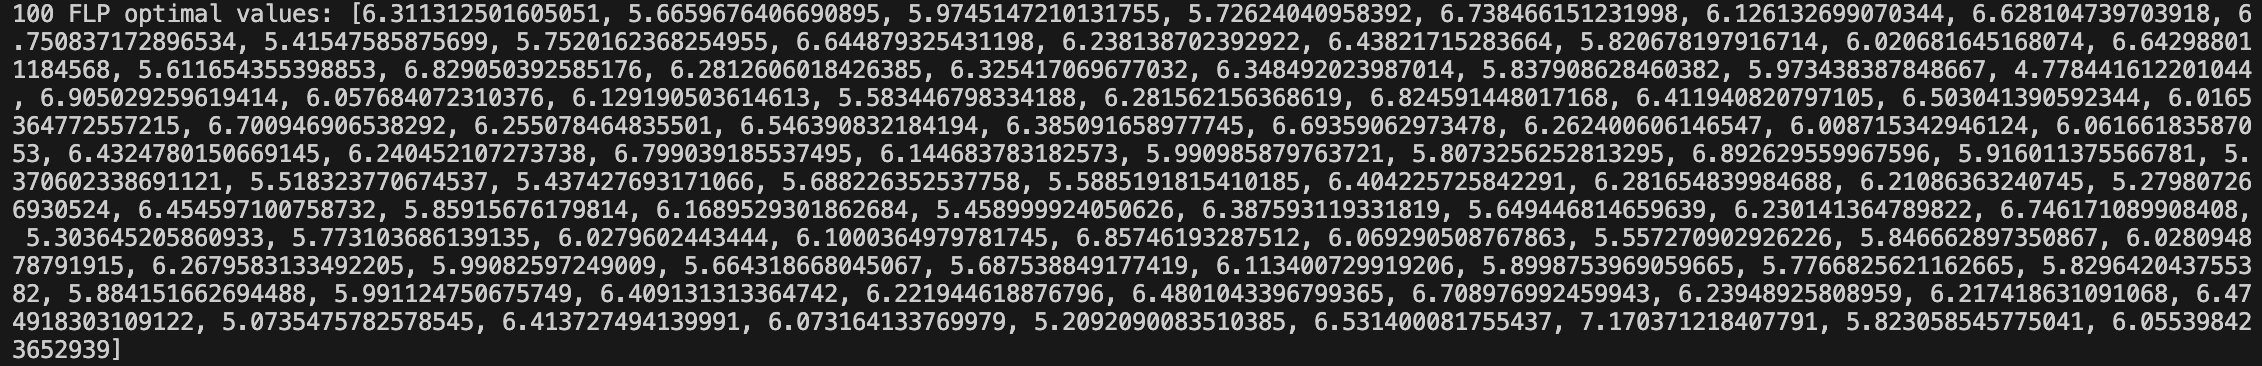
\includegraphics[width=1\linewidth]{FLP.png}
\end{figure}
For (FLP-LR), the 100 optimal values lie below:\\
\begin{figure}[H]
    \centering
    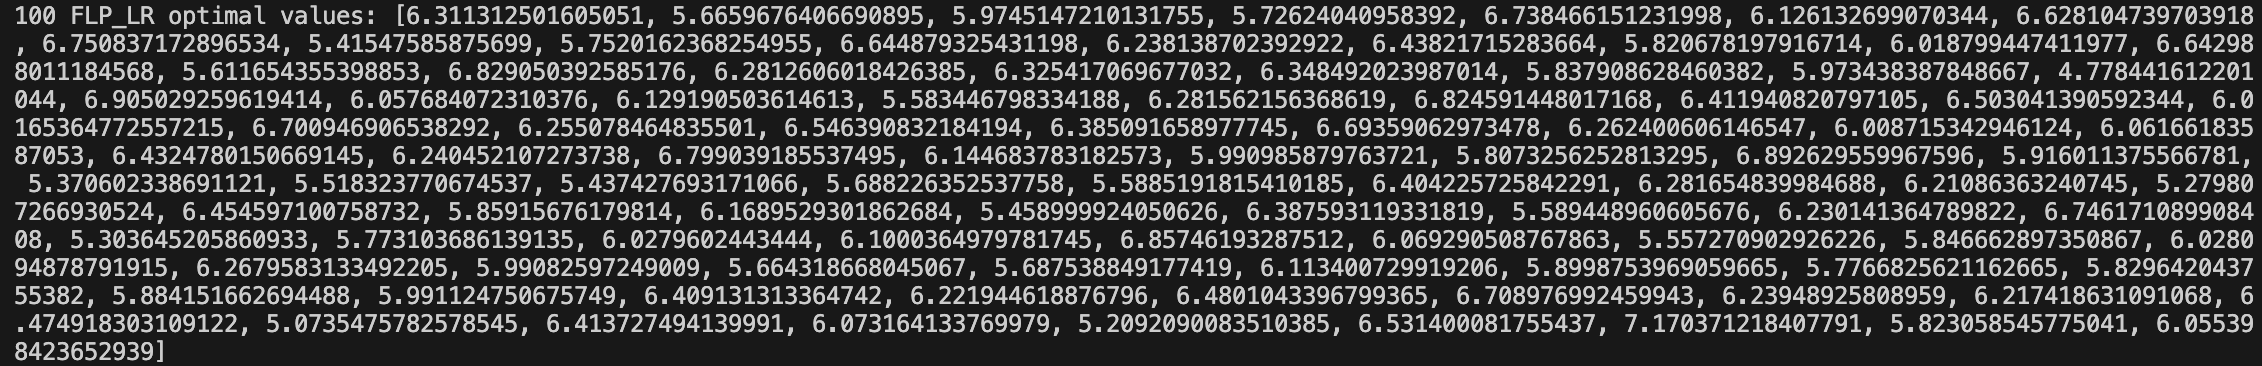
\includegraphics[width=1\linewidth]{FLP-LR.png}
\end{figure}

Second, we solve the facility location problem using (AFL) and solve the linear relaxation (AFL-LR) corresponding to (AFL).\\
We can solve this by following code:
\begin{minted}{python}
import gurobipy as gp
from gurobipy import GRB
from itertools import product 
import numpy as np

# Parameters
num_trials = 100

num_customers = 15
num_facilities = 10

AFL_vals = []
AFL_LR_vals = []

for t in range(num_trials):

  # Generate random data
  customers = [(np.round(np.random.rand(),2), np.round(np.random.rand(),2)) for i in 
  range(num_customers)]
  facilities = [(np.round(np.random.rand(),2), np.round(np.random.rand(),2)) for i in 
  range(num_facilities)]

  setup_cost = [1.0 for i in range(num_facilities)]
  cost_per_mile = 1.0

  # Compute distances
  def compute_distance(loc1, loc2):
      dx = loc1[0] - loc2[0]
      dy = loc1[1] - loc2[1]
      return np.sqrt(dx**2 + dy**2)

  # Compute parameters
  cartesian_prod = list(product(range(num_customers), range(num_facilities)))
  shipping_cost = {(c,f) : cost_per_mile*compute_distance(customers[c], facilities[f]) for c, f 
  in cartesian_prod}

  # AFL MIP model
  m_AFL = gp.Model("AFL")
  select = m_AFL.addVars(num_facilities, vtype=GRB.BINARY, name="Select")
  assign = m_AFL.addVars(cartesian_prod, ub=1, vtype=GRB.CONTINUOUS, name="Assign")

  m_AFL.addConstrs((gp.quicksum(assign[(c,f)] for c in range(num_customers)) <= num_customers*
  select[f] for f in range(num_facilities)), name="Setup2ship")
  m_AFL.addConstrs((gp.quicksum(assign[(c,f)] for f in range(num_facilities)) == 1 for c 
  in range(num_customers)), name="Demand")

  m_AFL.setObjective(select.prod(setup_cost) + assign.prod(shipping_cost), GRB.MINIMIZE)

  m_AFL.optimize()
  AFL_vals.append(m_AFL.ObjVal)

  # AFL Linear Relaxation 
  m_AFL_LR = gp.Model("AFL_LR")
  select = m_AFL_LR.addVars(num_facilities, ub=1, name="Select")
  assign = m_AFL_LR.addVars(cartesian_prod, ub=1, name="Assign")

  m_AFL_LR.addConstrs((gp.quicksum(assign[(c,f)] for c in range(num_customers)) <= num_customers*
  select[f] for f in range(num_facilities)), name="Setup2ship")
  m_AFL_LR.addConstrs((gp.quicksum(assign[(c,f)] for f in range(num_facilities)) == 1 for c 
  in range(num_customers)), name="Demand")

  m_AFL_LR.setObjective(select.prod(setup_cost) + assign.prod(shipping_cost), GRB.MINIMIZE)

  m_AFL_LR.optimize()
  AFL_LR_vals.append(m_AFL_LR.ObjVal)

print(len(AFL_vals), "AFL optimal values:", AFL_vals)
print(len(AFL_LR_vals), "AFL_LR optimal values:", AFL_LR_vals)  
\end{minted}
After running this program, we obtain the optimal values to (AFL) and (AFL-LR).\\
For (AFL), the 100 optimal values lie below:\\
\begin{figure}[H]
    \centering
    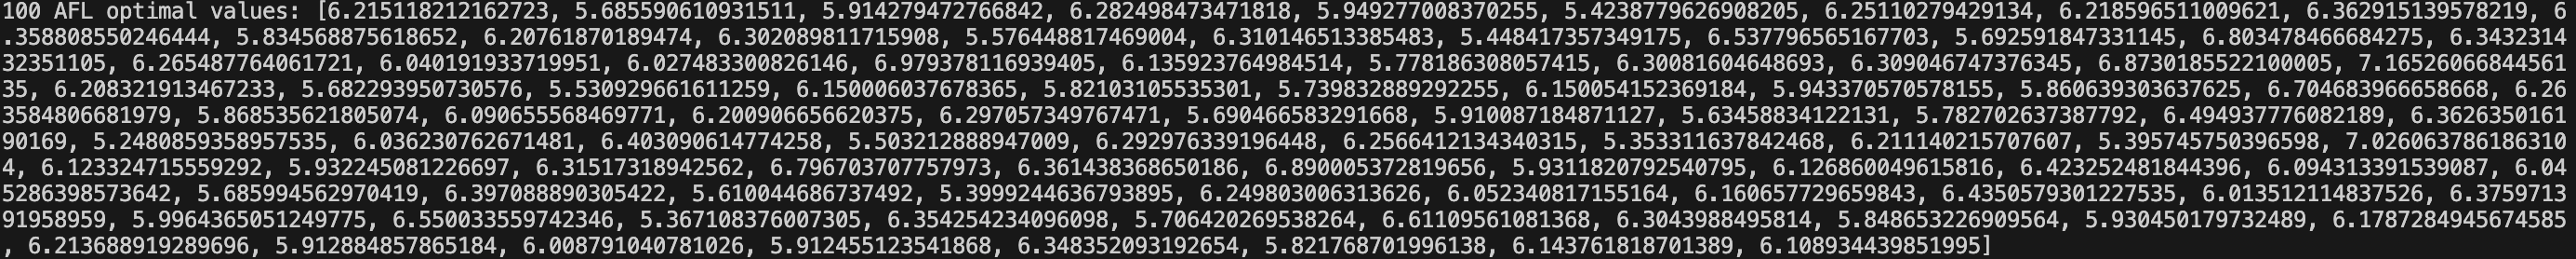
\includegraphics[width=1\linewidth]{AFL.png}
\end{figure}
For (AFL-LR), the 100 optimal values lie below:\\
\begin{figure}[H]
    \centering
    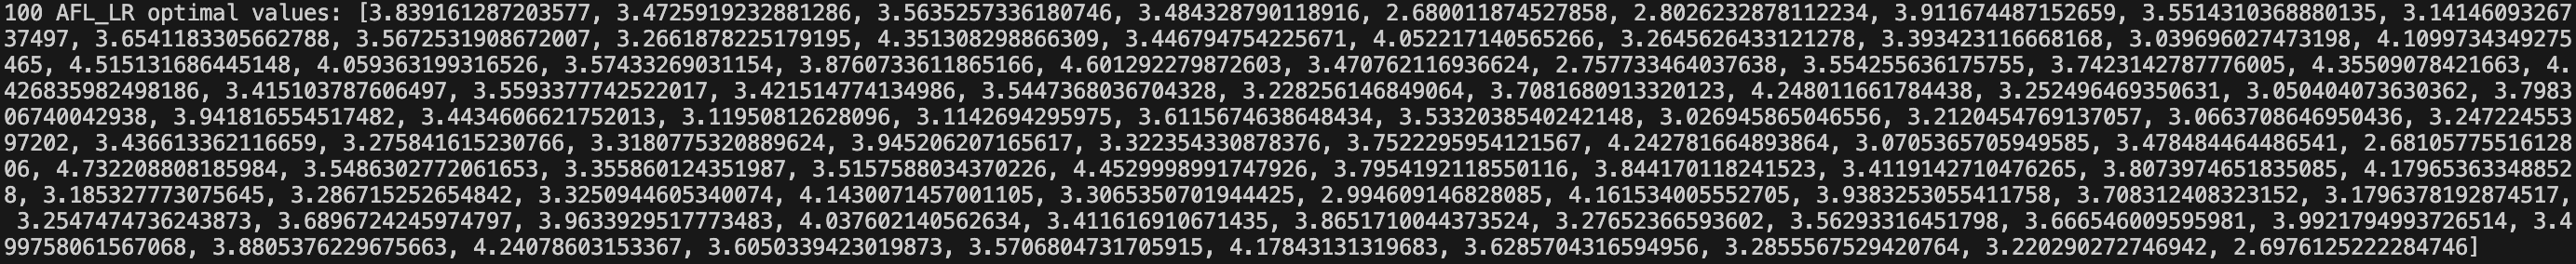
\includegraphics[width=1\linewidth]{AFL-LR.png}
\end{figure}

\subsection{Solution to Question(h)}
To compare and comment on the difference between the optimal values of all four optimization instances, we just need to count how often is (FLP-Val) equal to (FLP-LR-Val) and how often is (AFL-Val) equal to (AFL-LR-Val). To fulfill this purpose, we add 2 lines of code to the codes used in Question(g).\\
For (FLP) and (FLP-LR), the added code is:
\begin{minted}{python}
num_tight = sum(v1 == v2 for v1, v2 in zip(FLP_vals, FLP_LR_vals))
print("\nFLP tight in", num_tight, "trials")
\end{minted}
We can get the outcome below after 100 trials:
\begin{figure}[H]
    \flushleft
    
\includegraphics[width=0.25\linewidth]{FLP-Often.png}
\end{figure}
Similarly,for (AFL) and (AFL-LR), the added code is:
\begin{minted}{python}
num_tight = sum(v1 == v2 for v1, v2 in zip(AFL_vals, AFL_LR_vals))
print("\nAFL tight in", num_tight, "trials")
\end{minted}
We can get the outcome below after 100 trials:
\begin{figure}[H]
    \flushleft
    
\includegraphics[width=0.25\linewidth]{AFL-Often.png}
\end{figure}
All in all, from what we have done before, we can conclude that the difference between the optimal values of (FLP) and (FLP-LR) is small. In this way, we can consider (FLP-Val) and (FLP-LR-Val) as the same. However, when it comes to (AFL) and (AFL-LR), (AFL-Val) is totally different from (AFL-LR-Val).In this way, we cannot consider (AFL-Val) and (AFL-LR-Val) as the same.

\subsection{Solution to Question(i)}
The goal of this question is to formulate a capacitated facility location problem (CFLP) as a MILP and write down the linear relaxation.\\
The key difference between (CFLP) and the regular (FLP) is that each facility now has a limited capacity that constrains the number of customers it can serve.\\
To write the (CFLP), we simply add a constraint:
\begin{align*}
    \text{min} \quad &\sum_{j=1}^n c_jy_j+\sum_{i,j=1}^{m,n} d_{i,j}x_{i,j}\\
    \text{s.t.}\quad &\sum_{j=1}^n x_{i,j}=1 \qquad\text{for all} \quad i\\\tag{CFLP}
    &x_{i,j} \leq y_j \qquad\text{for all} \quad i,j\\
    &\sum_{i=1}^m x_{i,j} \leq r_j y_j\\
    &0\leq x_{i,j}\leq 1 ,y_{j}\in \left\{0,1\right\} .
\end{align*}

To write the linear relaxation of (CFLP), we simply replace the $y_j$ binary constraints with $0 \leq y_j \leq 1$ box constraints.\\
\begin{align*}
    \text{min} \quad &\sum_{j=1}^n c_jy_j+\sum_{i,j=1}^{m,n} d_{i,j}x_{i,j}\\
    \text{s.t.}\quad &\sum_{j=1}^n x_{i,j}=1 \qquad\text{for all} \quad i\\\tag{CFLP-LR}
    &x_{i,j} \leq y_j \qquad\text{for all} \quad i,j\\
    &\sum_{i=1}^m x_{i,j} \leq r_j y_j\\
    &0\leq x_{i,j}\leq 1\\
    &0\leq y_{j}\leq 1 
\end{align*}


\subsection{Solution to Question(j)}
From question(i) we know that what we need to do is just add a constraint.\\
To formulate this, we introduce a new parameter capacity that indicates the maximum number of customers that can be served by each facility.\\
Then we add the following new constraint to the (FLP) MILP model:
\begin{minted}{python}
# Capacity constraint 
m.addConstr(sum(assign[(c,f)] for c in customers) <= capacity*select[f] for f in facilities)    
\end{minted}
This requires that the total number of customers assigned to a facility is less than the capacity if the facility is selected.\\
After 100 trials, we obtain the following outcome:
\begin{figure}[H]
    \flushleft
    
\includegraphics[width=0.25\linewidth]{CFLP-Often.png}
\end{figure}

\section{Traveling Salesman Problem}
\subsection{Solution to Question(a)}
To solve this question, we realized we would need to loop through the tour to calculate the total distance. To look up the distances between cities, we would need their indices to index into the distance matrix. So we decided to convert the city tour into a list of indices by subtracting $1$ from each city number.\\
Next, to loop through the tour, we knew we would need to access the next index after the current one. So we decided to use \pyth{'np.roll'} to shift the index list by $-1$ to get the next city index.
Then, we indexed the distance matrix using these index lists to get the actual distances between consecutive cities.
Finally, we summed all the retrieved distances to get the total tour distance. We also handled the edge case from last city back to first city.\\
The code is as follows:
\begin{minted}{python}
# Distance calculation
def calculate_tour_distance(tour, dist_matrix):
    indices = np.array(tour) - 1
    dist = dist_matrix[indices, np.roll(indices, -1)]
    return dist.sum()
\end{minted}
The \pyth{'calculate_tour_distance'} function calculates the total length of a city tour. It takes two parameters: \pyth{'tour'}, which is a list containing the order of cities, and \pyth{'dist_matrix'}, which is the matrix of distances between cities. This function first subtracts 1 from the city indices in the \pyth{'tour'} to match array indexing. Then, it uses NumPy array operations to calculate the distances between adjacent cities and returns the sum of these distances as the total tour length.

\subsection{Solution to Question(b)}
To solve this question, we knew we needed to modify the tour to create a candidate. Reversing a section of the tour seemed like a good option for perturbation.We decided to make a copy of the tour first to avoid modifying the original tour.\\
Next, we needed to randomly select two indices to define the section to reverse. \pyth{'np.random.choice'} is useful for sampling indices without replacement. Then, we used \pyth{'np.flip'} to neatly reverse the slice between the two selected indices. Finally, we return the new candidate tour with the reversed section.\\
The code is as follows:
\begin{minted}{python}
# Tour perturbation
def generate_candidate(tour):
    n = len(tour)
    i, j = sorted(np.random.choice(range(n), 2, replace=False))
    candidate = tour.copy()
    candidate[i:j] = np.flip(candidate[i:j])
    return candidate
\end{minted}
The \pyth{'generate_candidate'} function is responsible for creating a candidate tour by perturbing the current tour. It randomly selects two cities ($i$ and $j$) from the tour and reverses the order of the cities between them, creating a new tour. 

\subsection{Solution to Question(c)}
To solve this question, we first initialized the algorithm by randomly generating a tour and setting an initial temperature. Then, we knew we would need a loop where each iteration generates and evaluates a candidate tour. Inside the loop, we call the \pyth{'generate_candidate'} function to get a new candidate tour. Next, we calculate the tour lengths for the current and candidate tours to get the change in cost \pyth{delta_f}.\\
Using \pyth{delta_f} and the temperature \pyth{T}, we probabilistically decide whether to move to the candidate tour or stay at the current tour. We also track the best tour found so far within the loop. Finally, we reduce the temperature \pyth{T} gradually according to the annealing schedule. After many iterations, the algorithm converges to a good tour.\\
The code is as follows:
\begin{minted}{python}
# (c) Simulated annealing
def simulated_annealing(dist_matrix, max_iters=10000, T0=100, eta=0.99):

    n = len(dist_matrix)
    current = np.random.permutation(n) + 1

    best = current.copy()
    f_curr = calculate_tour_distance(current, dist_matrix)
    T = T0

    for i in range(max_iters):
        candidate = generate_candidate(current)
        f_cand = calculate_tour_distance(candidate, dist_matrix)

        delta_f = f_cand - f_curr
        if delta_f < 0 or np.random.rand() < math.exp(-delta_f / T):
            current = candidate
            f_curr = f_cand

        if f_cand < calculate_tour_distance(best, dist_matrix):
            best = candidate

        T *= eta

    return best
\end{minted}
The \pyth{'simulated_annealing'} function is the core of the entire solution. It takes the distance matrix \pyth{'dist_matrix'} and several algorithm parameters, including the maximum number of iterations, initial temperature (\pyth{T0}), and cooling rate (\pyth{eta}). Initially, it randomly generates a starting tour and uses the simulated annealing algorithm to find a shorter tour.\\
In each iteration, it generates a new candidate tour and calculates the total length of the new tour.\\
It compares the difference (\pyth{delta_f}) between the current tour and the candidate tour's length with the temperature (\pyth{T}) to decide whether to accept the new tour. If the new tour is shorter or with a certain probability, even if it's longer, it may be accepted to explore the search space.\\
It also keeps track of the best tour found.\\
The temperature (\pyth{T}) is reduced at each iteration to simulate the annealing process.\\

\subsection{Solution to Question(d)}
To test the implementation in Question(c), we first generate random coordinates for 50 cities and then calculate the distance matrix using the \pyth{'pairwise_distances'} function.\\
Then, we print out the distance matrix that represents the distances between the randomly generated cities for inspection.\\
Finally, we run the simulated annealing algorithm to find the best city tour, and then print out the found tour and its total length.\\
The code is as follows:
\begin{minted}{python}
# (d) Generate random 50 city instance and run simulated annealing

num_cities = 50
cities = np.random.rand(num_cities, 2)
dist_matrix = pairwise_distances(cities)

print(f"Distance matrix for {num_cities} randomly generated cities:")
print(dist_matrix)

best_tour = simulated_annealing(dist_matrix)

print(f"\nBest tour found by simulated annealing:")
print(best_tour)

best_distance = calculate_tour_distance(best_tour, dist_matrix)
print(f"\nDistance of the best tour: {best_distance}")
\end{minted}
After running this program, we have the following outcome:
\begin{figure}[H]
    \centering
    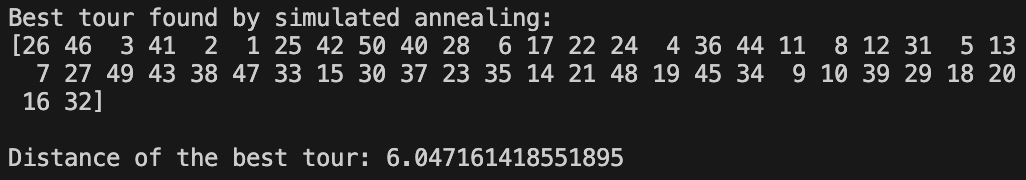
\includegraphics[width=0.75\linewidth]{TSP(Optimal).png}
\end{figure}


\subsection{Solution to Question(e)}
We use \pyth{'matplotlib'} to create a visualization. We plot the cities as points, and then connect them in the order specified by the best tour with red lines, forming a visual representation of the city tour.\\
The code is as follows:
\begin{minted}{python}
# Visualization
plt.plot(cities[:, 0], cities[:, 1], 'o')
for i in range(len(best_tour)):
    plt.plot([cities[best_tour[i] - 1, 0], cities[best_tour[(i + 1) % num_cities] - 1, 0]],
             [cities[best_tour[i] - 1, 1], cities[best_tour[(i + 1) % num_cities] - 1, 1]], 'r-')

plt.show()
\end{minted}
After running this program, we have the following outcome:
\begin{figure}[H]
    \centering
    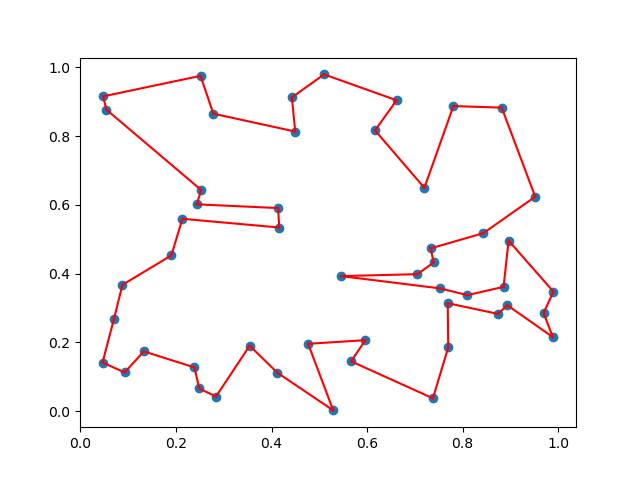
\includegraphics[width=0.5\linewidth]{Figure_1.png}
\end{figure}
From the outcome, we can find that this tour doesn't have edges that intersect. Therefore, the outcome is an optimal tour.

\subsection{Solution to Question(f)}
The key modification is in the \pyth{'generate_candidate'} function. Instead of reversing a subsequence of cities, we now randomly select two indices $i$ and $j$, and we swap the positions of the cities at these indices in the \pyth{'candidate tour'}. This creates a different proposal rule where you swap two cities while keeping all other cities intact. \\
The code is as follows:
\begin{minted}{python}
# Tour perturbation (alternative rule: swapping two indices)
def generate_candidate_swap(tour):
    n = len(tour)
    i, j = np.random.choice(range(n), 2, replace=False)
    candidate = tour.copy()
    candidate[i], candidate[j] = candidate[j], candidate[i]
    return candidate
\end{minted}
After running this modified program, we have the following outcome:
\begin{figure}[H]
    \centering
    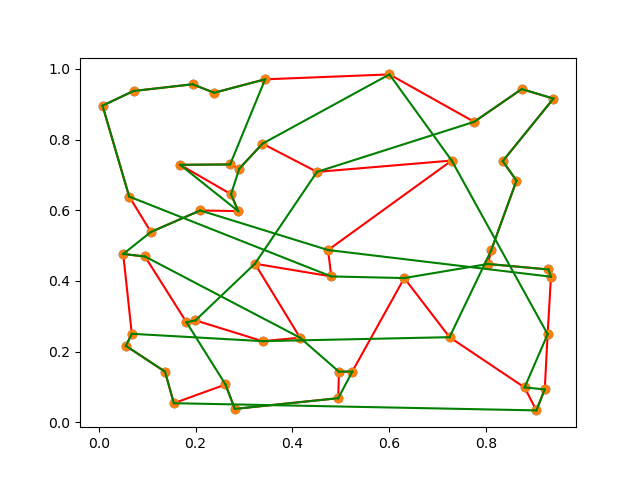
\includegraphics[width=0.5\linewidth]{Figure_2.png}
\end{figure}
The figure means that the new proposal rule also obtains an optimal tour.
Then we have two distance of best tour from the reversing and swapping:
\begin{figure}[H]
    \centering
    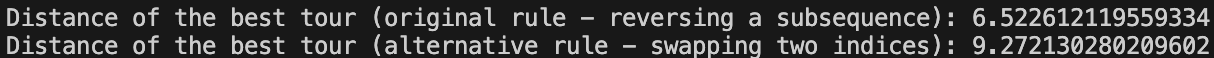
\includegraphics[width=1\linewidth]{TSP(Comparison).png}
\end{figure}
Comparing with the two proposal rules, we can find that reversal finds slightly shorter tours. However, after several trials, we can find that both methods work well to explore the search space and converge to good solutions.

\bibliography{bibliography}
\end{document}